\begin{frame}
\frametitle{Aufgabe 2}
\framesubtitle{Bode Diagramm}
    \begin{itemize}
        \item Bode Diagramm: Auftragung Amplitude über Frequenz
        \item Visualisierung von Dämpfung
    \end{itemize}
\end{frame}
\begin{frame}
\frametitle{Aufgabe 2}
\framesubtitle{Frequenzfilter}
    \begin{itemize}
        \item Hoch-,Tief-,Bandpassfilter
        \item Unterdrückung von Frequenzbereichen
        \item Ordnung gibt an wie stark die Dämpfung ausfällt: 1. Ordnung:
        $6db$ pro Oktave, 2. Ordnung $12dB$ pro Okatave etc.
        \item nichtlineares Verhalten
    \end{itemize}
\end{frame}
\begin{frame}
\frametitle{Aufgabe 2}
\framesubtitle{Tiefpassfilter 1. Ordnung}
\begin{figure}[H]
\begin{center}
        \includegraphics[scale=0.2]{./img/2a_bode_schaltbild.png}
\end{center}
\end{figure}
\begin{itemize}
    \item $3dB$-Frequenz: Abfall des Signals
    $\frac{U_{in}}{U_{out}}=\frac{1}{\sqrt{2}}$
    \item Grenzfrequenz
\end{itemize}
\end{frame}
\begin{frame}
\frametitle{Aufgabe 2}
\framesubtitle{Tiefpass 1. Ordnung}
\begin{figure}[H]
\begin{center}
        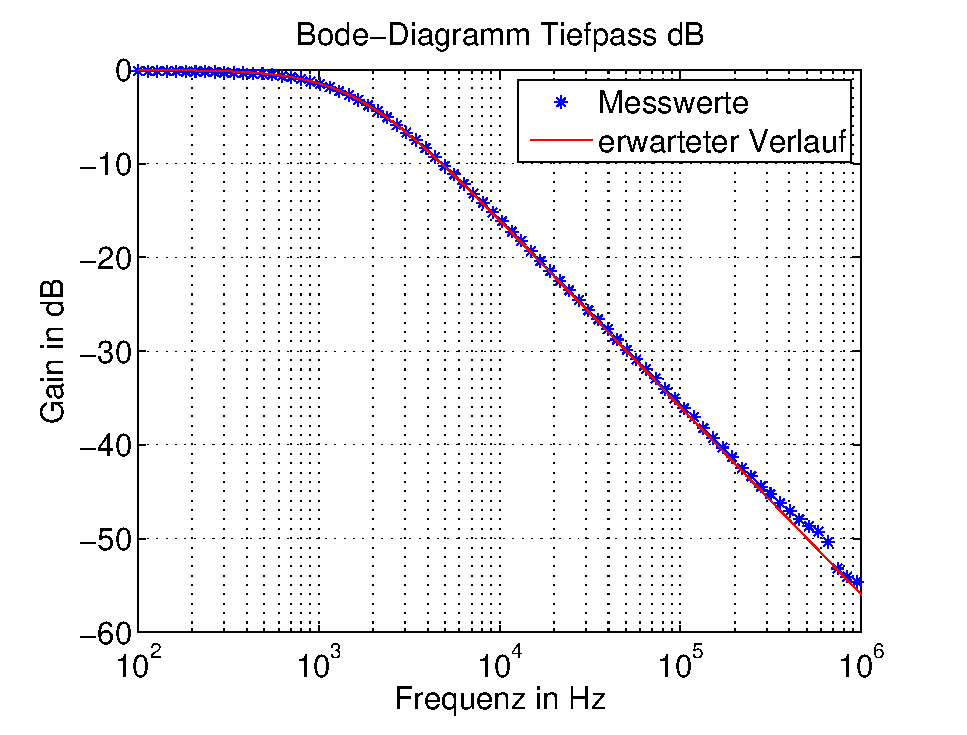
\includegraphics[scale=0.3]{./img/2a_bode_tief_dB.eps}
\end{center}
\end{figure}
\end{frame}
\begin{frame}
\frametitle{Aufgabe 2}
\framesubtitle{Tiefpass 1. Ordnung}
\begin{figure}[H]
\begin{center}
        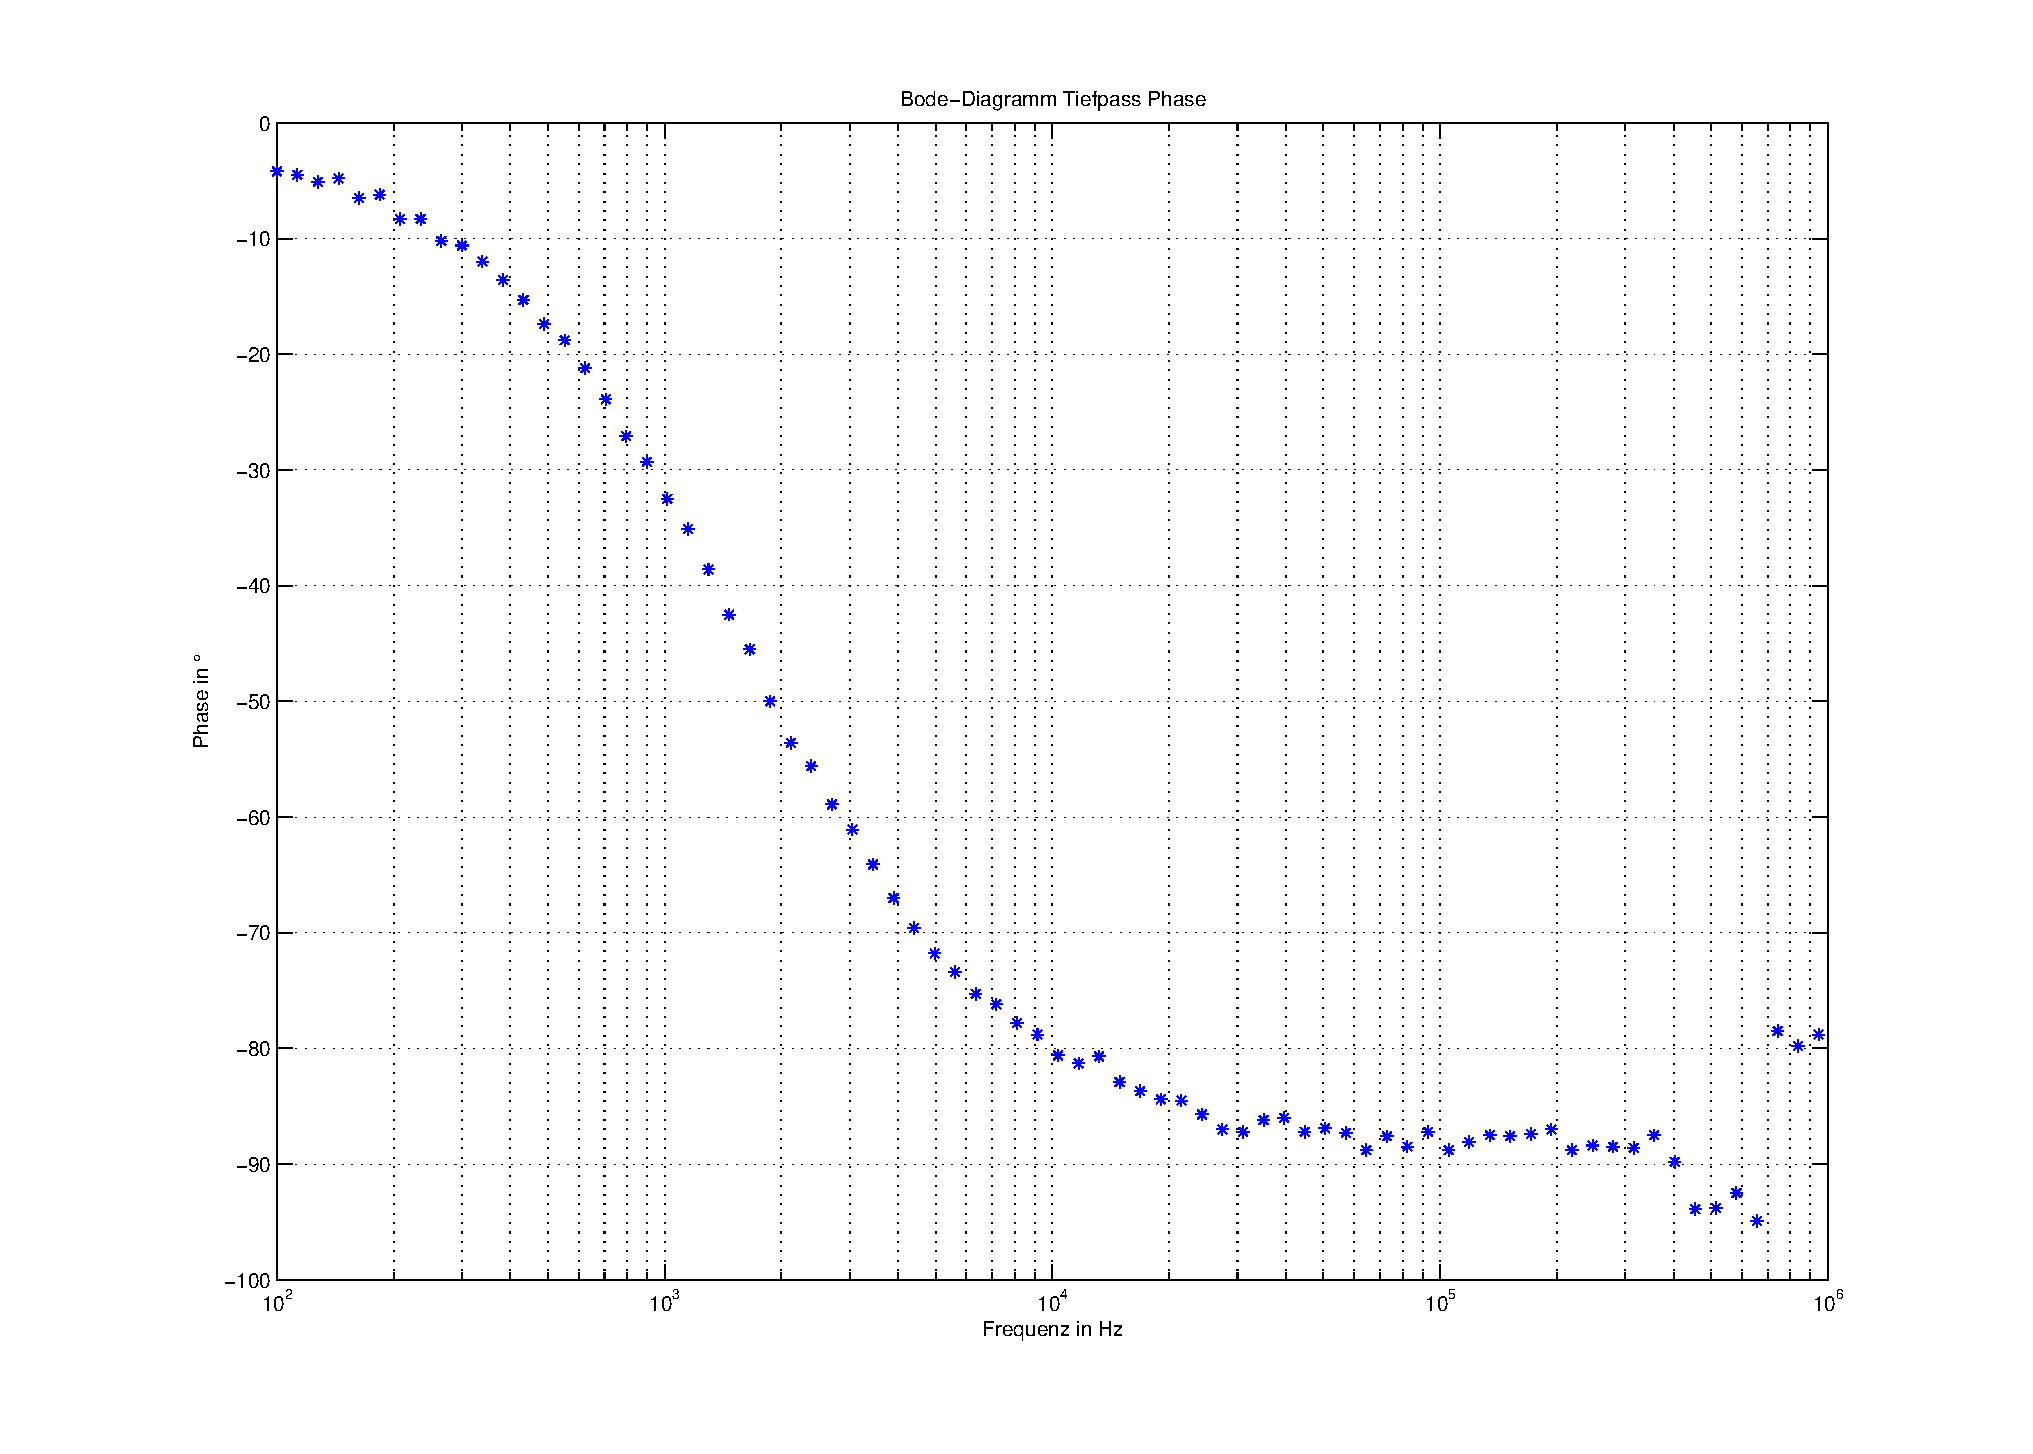
\includegraphics[scale=0.3]{./img/2a_bode_tief_phase.eps}
\end{center}
\end{figure}
\end{frame}
\begin{frame}
\frametitle{Aufgabe 2}
\framesubtitle{Tiefpass 1. Ordnung}
\begin{figure}[H]
\begin{center}
        \includegraphics[scale=0.3]{./img/2a_bode_tief_UoutUin.eps}
\end{center}
\end{figure}
\end{frame}

\begin{frame}
\frametitle{Aufgabe 2}
\framesubtitle{AC-Modus des Oszilloskops}
\begin{figure}[H]
\begin{center}
        \includegraphics[scale=0.2]{./img/2c_Testsignal_1.png}
\end{center}
\end{figure}
\begin{itemize}
    \item Testsignal: Dreiecksspannung + Sinussignal
    \item Problem: Schwierigkeit bei automatischer Bestimmung der
    Amplitude - Sinus ist "schräg" und wandert
\end{itemize}
\end{frame}

\begin{frame}
\frametitle{Aufgabe 2}
\framesubtitle{AC-Modus des Oszilloskops}
\begin{itemize}
    \item Lösung 1: Vorschaltung eines Hochpassfilters
    \item Dreickspannung ist niedrigfrequentes Signal $\rightarrow$ wird herausgefilter
\end{itemize}
\begin{figure}[H]
    \begin{center}
            \includegraphics[scale=0.2]{./img/2c_Dreieck.png}
    \end{center}
\end{figure}
\end{frame}
\begin{frame}
\frametitle{Aufgabe 2}
\framesubtitle{Ac-Modes des Oszilloskops}
\begin{itemize}
    \item Lösung 2: Eingang auf AC-Modus
    \item eingebauter Hochpassfilter 
    \item Verwendung zum Filtern niedrigfrequenter Störungen
\end{itemize}
\begin{figure}[H]
\begin{center}
        \includegraphics[scale=0.2]{./img/2c_Testsignal_AC.png}
\end{center}
\end{figure}

\end{frame}
